\section{Introduction}
\label{sec:introduction}
% TODO in each sections deforestation, emissions and ecosystem service mention research gaps

\subsection{Tropical forest}
	\begin{figure}[h]
		\centering
		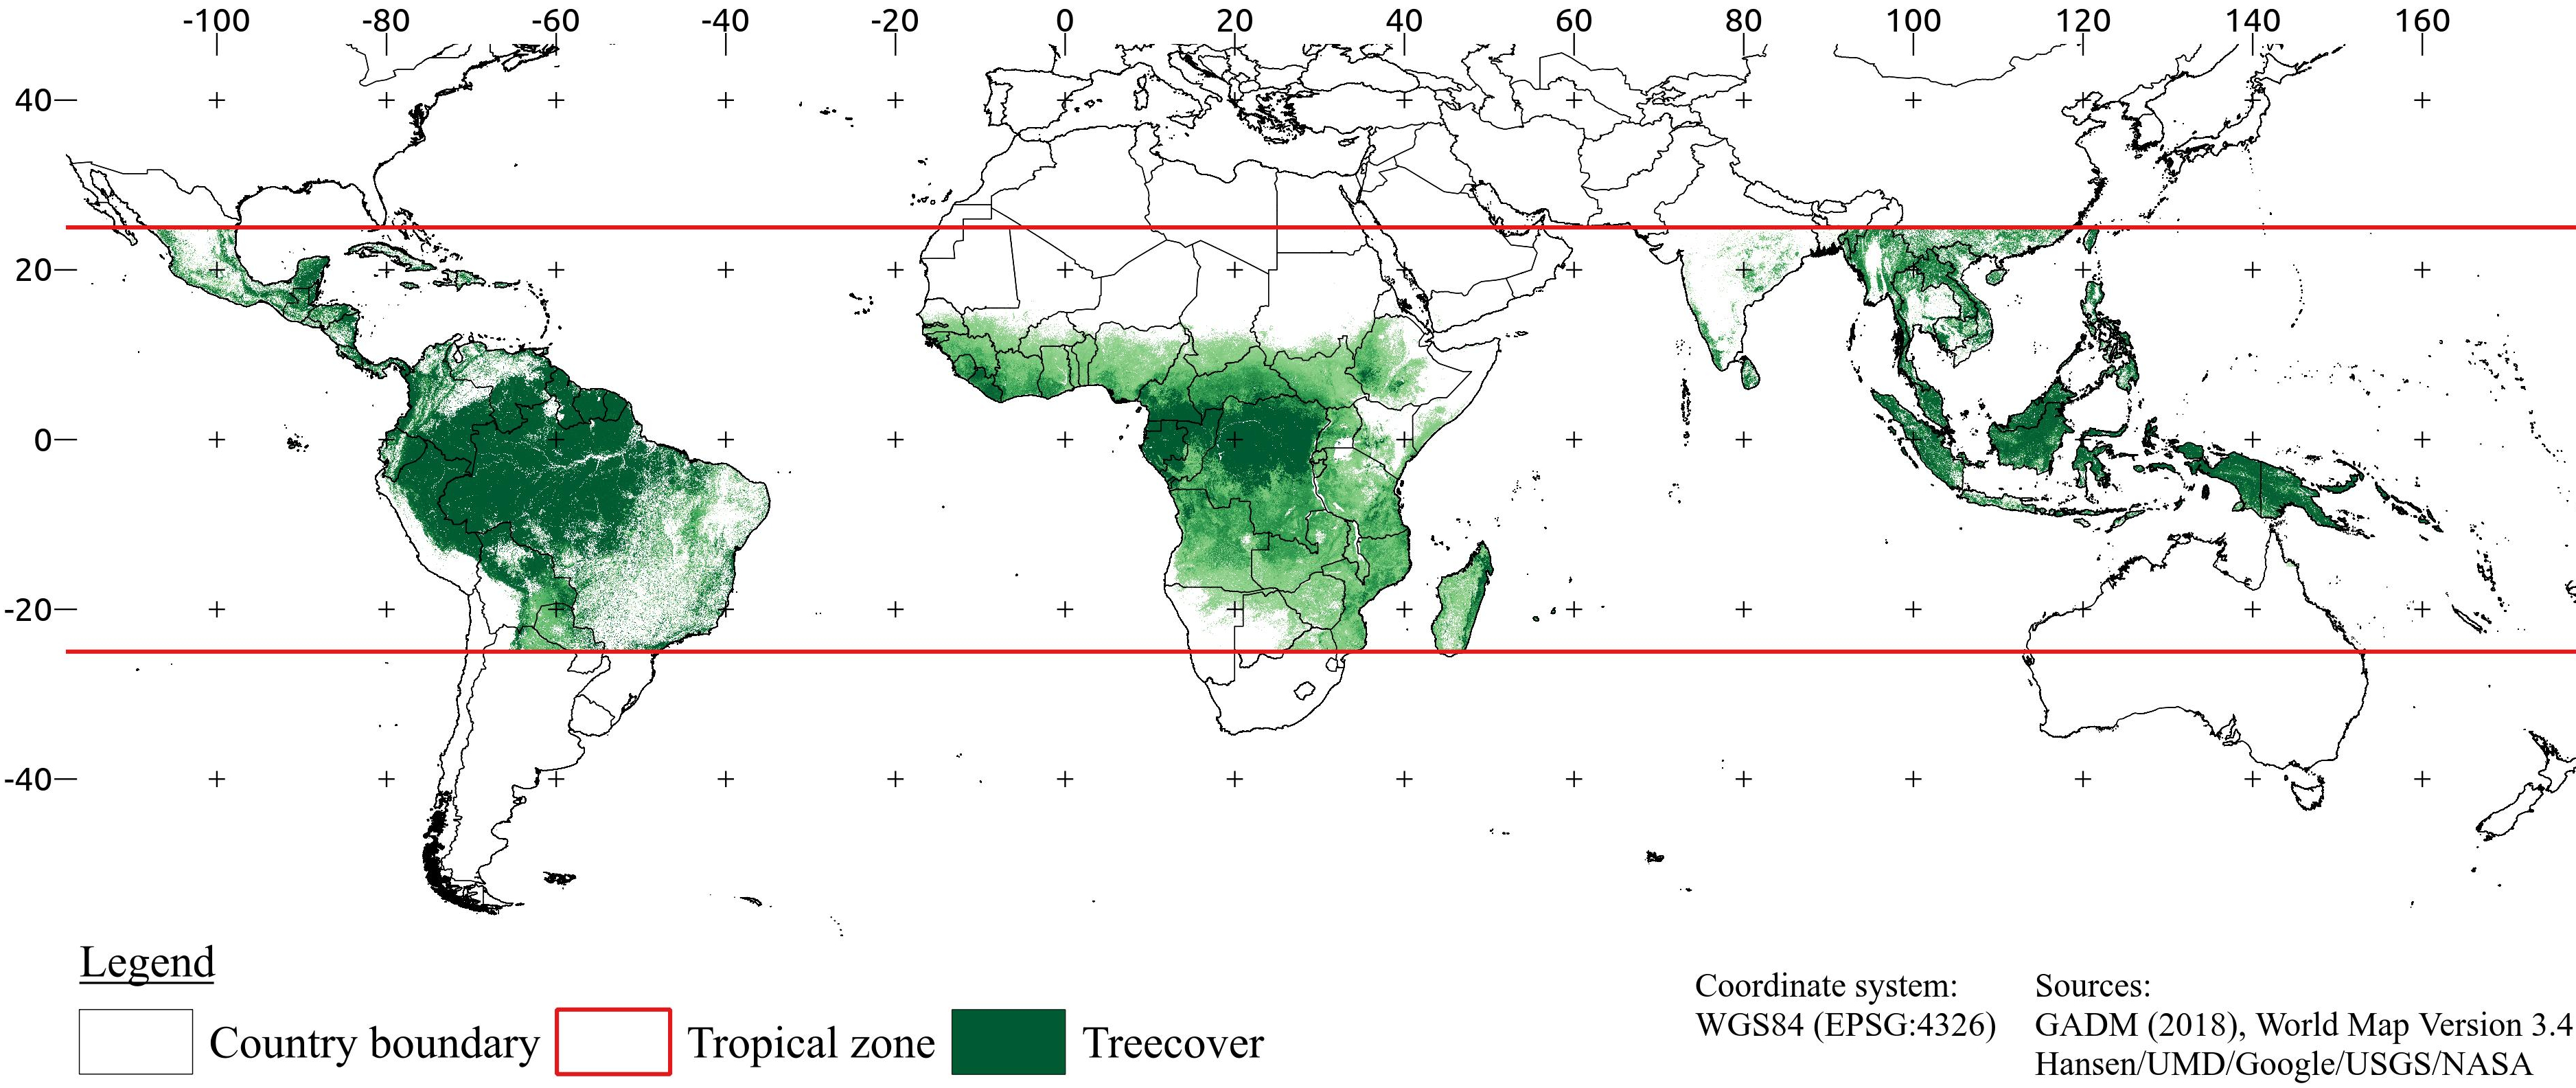
\includegraphics[scale=0.95]{img/intro_overview_frameless}
		\caption[Study extent]{Geographic tropical zone framed red and the tropical forest}
		\label{fig:intro_overview}
	\end{figure}

	\subsubsection{Current state}
		\lipsum[1-3]

	\subsubsection{Contribution to climate}
	\subsubsection{Forest definitions}

\subsection{Deforestation}
	{\color{red} Gaps no spatial explicit knowledge on direct deforestation drivers (amount, pattern, cattle ranching/cropland, urbanization)}

	{\color{red} Contribution of deforestation drivers on ghg emissions, no knowledge on soil organic carbon emissions} 
	\subsubsection{Land use and land cover change}
	\subsubsection{Drivers of deforestation}
	\subsection{Emissions trough deforestation}
	\subsubsection{Removal of AGB}
	\subsubsection{Soil organic carbon change and soil dynamics}

\subsection{Ecosystem services}
	{\color{red} till now only estimates of losses no balance estimate} 
	\subsubsection{Ecosystem service values}
	\subsection{Research objective and questions}
